\documentclass[12pt,a4paper,oneside]{article}
\usepackage{cmap}
\usepackage[T2A]{fontenc} 
\usepackage[utf8]{inputenc}
\usepackage[english, russian]{babel}

\usepackage{amsmath,amsfonts,amssymb,amsthm,mathtools}

\usepackage{tikzsymbols}
\usepackage{marvosym}

\usepackage{graphicx}

\usepackage{hyperref}

\title{firstex}
\author{DarinaShebzukhova }
\date{February 2017}

\begin{document}
\maketitle
\section{А напиши-ка 10 фактов о себе!}
\begin{enumerate}
\item Меня зовут Дарина. Хотя часто приходится быть Тариной, Кариной, Мариной, а еще Дианой, Даяной ну и Дашей, в конце концов. \Smiley
\item Уже вторым пунктом хочется сказать, как я люблю сон. Вообще во время сна происходит много полезных процессов, поэтому неохотно им жертвую. 
\item Отсюда логичным образом вытекает любовь к кофе \Coffeecup, хотя должного эффекта от него давненько не помню.
\item За последние дни много раз хотелось если не убивать, то что-то около того, потому что Тех не устанавливался раз 6 по несколько часов создавая вид бурной деятельности. К слову, он так этого и не сделал- \Sadey.
\item Эта зима была создана для лыж и борда, а я каждый раз недоумеваю, почему не воспользовалась возможностями научиться.
\item С каждым пунктом факты все тяжелее придумываются - факт! 
\item И Алло! надо делать все вовремя- вот этого я совсем не умею. и никакой тайменджмент здесь не поможет)
\item Я все чаще влюбляюсь в мультфильмы. Вот сегодня был "песнь моря". Если не смотрели - советую.
\item Попросила несколько фактов о себе со стороны, поняла, что люди хороши. \Heart
\item Писать про себя - не самое легкое и любимое. и извините, что читать было невесело.

\end{enumerate}


\section {5 любимых формул}


\begin{equation}\label{t1} 
f(x)= \dfrac{1} {\sigma *\sqrt{2 \pi}}\cdot {e^{-{\dfrac{(x-\mu)^2}{2\sigma^2}}}\tag{\ae}
\end{equation} 

\begin{equation}\label{t2}
\sin{\alpha}\pm \sin{\beta} = 2 \cdot \sin{\dfrac{\alpha \pm \beta}{2}} \cdot \cos{\dfrac{\alpha \mp \beta}{2}}\tag{\ae\ae}
\end{equation}

\begin{equation} \label{t3}
\Phi(x) = \dfrac {2}{\sqrt{\pi}} \int\limits_0^{+\infty} e^{-t^2}dt\tag{\ae\ae\ae}
\end{equation}

\begin{equation} \label{t4}
\lim\limits_{x \to 0}\dfrac{\ln{(1+x)}}{x}=1\tag{\ae\ae\ae\ae}
\end{equation}

\begin{equation} \label{t5}
\det\begin{bmatrix}a_{11} & \dots & a_{1n} \\
\vdots & \ddots & \vdots \\
a_{m1} & \dots & a_{mn}
\end{bmatrix} = \det\begin{bmatrix}a_{11} & \dots & a_{m1} \\
\vdots & \ddots & \vdots \\
a_{1n} & \dots & a_{mn}\end{bmatrix}\tag{\ae\ae\ae\ae\ae}
\end{equation}
\subsection{и одна не фонтан}
\begin{equation} \label{t6}
G= \sum\limits_{i=1}^n p_i \cdot q_{i+1} - \sum\limits_{i=1}^n p_{i+1}\cdot q_i\tag{\ae\ae\ae\ae\ae\ae}
\end{equation}
\subsection{А что вдруг они?}
Ну \ref{t1} - это функция плотности нормального распределения, оно всеми любимо и часто даёт приятные результаты (ну поприятнее, чем в других распределениях);\\
\ref{t2} - а тут эхом отдается школьная симпатия к тригонометрии;\\
\ref{t3} - Алиса пару раз говорила, что я, очевидно, люблю эту формулу, раз часто вспоминаю);\\
\ref{t4} - ну замечательный же? он и его друзья вообще прелести, я щитаю
\ref{t5} - вспоминая Артамоновых;\\
\ref{t6} - а тут стараясь забыть количество раз,сколько я забывала порядки индексов и путалась в решении.

\section{фото же надо приложить}
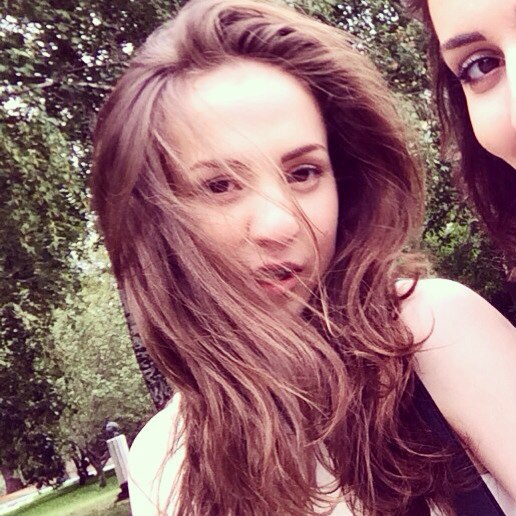
\includegraphics[width= 10 cm]{fotachka.jpg}


\end{document}